% !TeX root = 190227.tex
\section{Веб}
\begin{frame}[t]{Сетевые уровни}
	Сетевая модель OSI (кусочек):
	
	\begin{center}
		\begin{tabular}{clll}
		\hline
		Номер & Название &  Пример & Что шлёт пример \\\hline
		7 & Прикладной & HTTP & Веб-запросы \\
		4 & Транспортный & TCP & Потоки байт \\\hline
		3 & Сетевой & IPv4, IPv6 & Пакеты байт \\
		2 & Канальный & Ethernet, DSL & Пакеты байт \\
		1 & Физический & & Поток бит \\\hline
		\end{tabular}
	\end{center}
	
	\begin{itemize}
		\item Нижнему уровню всё равно, кто наверху
		\item Верхний уровень старается не пользоваться информацией про нижний
			\begin{itemize}
			\item HTTP нужен TCP или что-то похожее
			\item HTTP неважно, IPv4 или IPv6
			\end{itemize}
	\end{itemize}
\end{frame}

\begin{frame}[t]{NAT}
	\begin{center}
		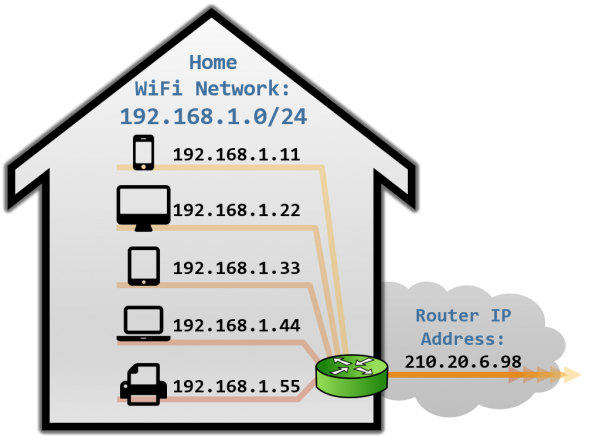
\includegraphics[scale=0.3]{nat-home.png}
		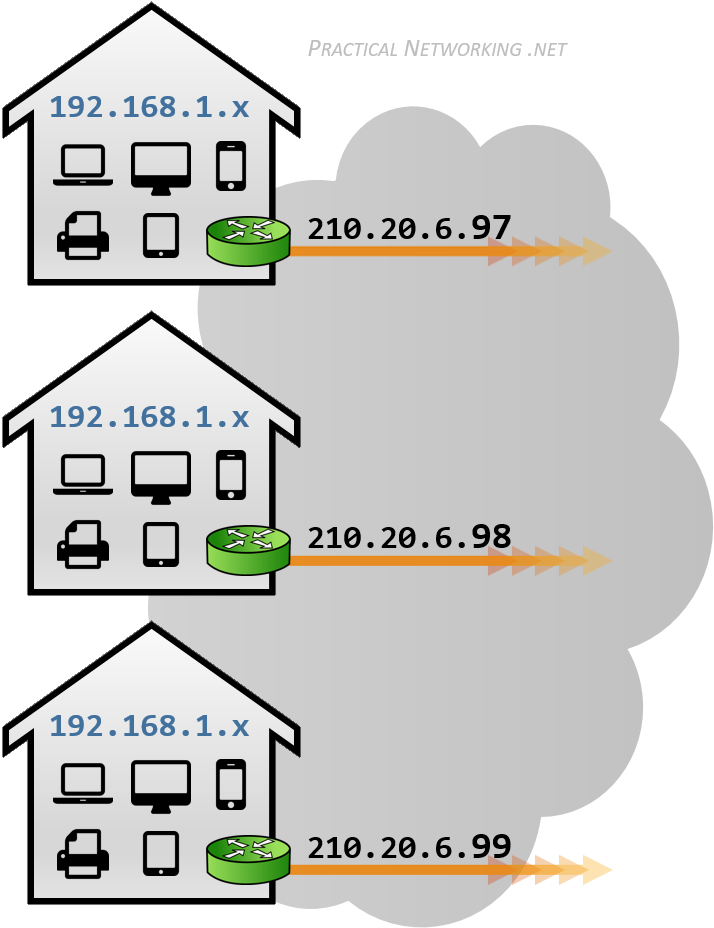
\includegraphics[scale=0.3]{nat-homes.png}
	\end{center}
	Источник: \href{https://www.practicalnetworking.net/series/nat/why-nat/}{www.practicalnetworking.net/series/nat/why-nat/}
\end{frame}

\begin{frame}[t]{Токены доступа}
	\begin{itemize}
		\item Технически можно выдать сколько угодно на пользователя и приложение
		\item Можно отслеживать соблюдение правил
		\item Легко банить, легко отзывать только один токен
		\item Никогда не храните в коде!
			\begin{itemize}
			\item Кто нашёл токен "--- действует от вашего имени
			\item Код можно случайно кому-нибудь отправить <<как пример>>
			\item Код можно выложить на GitHub
			\item Храните в отдельном файле или переменных окружения
			\end{itemize}
	\end{itemize}
\end{frame}
